\documentclass[t]{beamer}
\usetheme{Warsaw}
\usecolortheme{seahorse}
\usepackage{array}
%\usepackage{graphicx}
\usepackage{amssymb,amsmath,mathrsfs,amsfonts}
%\usepackage[colorhighlight,display]{texpower}
%\usepackage{caption}
%\usepackage[all]{xy}
\usepackage{beamerthemesplit}
\mode<presentation>
%\usepackage{pause}
\usepackage{ulem}  % for strikethroughs
\usepackage{cancel} % for strikethroughs in math mode 
\usepackage{tikz}
\usepackage{calc}
\usetikzlibrary{shapes}
\usepackage{hyperref}
\hypersetup{pdfpagemode=FullScreen}
\usepackage{ifthen}
\usepackage{animate}
\usepackage{color}
\usepackage{type1cm}  % used for watermarking
\usepackage{eso-pic}  % used for watermarking


\theoremstyle{plain}
\newtheorem{prop}{Proposition}
\newtheorem{thm}[prop]{Theorem}
\newtheorem{lem}[prop]{Lemma}
\newtheorem{cor}[prop]{Corollary}
\theoremstyle{definition}
\newtheorem{dfn}{Definition}
\newtheorem{rem}[prop]{Remark}
\newtheorem{ex}{Example}[section]
%\newtheorem{note}{Note}[section]
\newtheorem{exercise}{Exercise}[section]
\newcommand{\nin}{\noindent}
\newcommand{\ds}{\displaystyle}
\renewcommand{\figurename}{Figure \arabic{figure}}



\renewcommand*\familydefault{\sfdefault} 




%%%%%%%%%%%%%%%%%%%%%%%%%%5
%%%%%%%%%%%%%%%%%%%%%%%%%%%%
%%%% some commands that have different meaning in the article/presentation modes

\newcommand{\vvfill}{\mode<presentation>{\vfill}  \mode<article>{\medskip}}   %vfill in presentation only
\newcommand{\sketchspace}{ 
\mode<article>{ \medskip\noindent{\textbf{Sketch:}} \vspace*{6cm} }
\mode<presentation>{ } 
}
\newcommand{\examplespace}{ 
\mode<article>{ \medskip\noindent{\textbf{Example:}} \vspace{6cm} }
\mode<presentation>{ } 
}
\newcommand{\artsmspace}{\mode<article>{\vspace*{2cm}} }  %small space in article mode
\newcommand{\artlargespace}{\mode<article>{\vspace*{6cm}} }  %large space in article mode

\newcommand{\dx}{\,dx}

\newcommand{\soln}{{\textbf{Solution: }}\,\,\,}
\newcommand{\disp}{\displaystyle}

\newcommand{\makedate}{\vvfill
\begin{picture}(10,10)  
\put(260,-20){\mbox{\tiny{\today}}}
\end{picture}
}

\newcommand{\pd}[2]{\dfrac{\partial#1}{\partial#2}}
\newcommand{\pD}[2]{\dfrac{\partial^2#1}{\partial#2^2}}
\newcommand{\pdd}[3]{\dfrac{\partial^2#1}{\partial#2 \partial#3}}


\normalem %stops the ulem package making all the emphs into underlines....
 
 
 
 \newcommand{\refandrev}[2]{
 \begin{small}
  \hspace{6cm}
  \begin{minipage}[r]{8cm}
  Stewart,    Chapter #1   \\
  Review:  \parbox[t]{6cm}{#2}
\end{minipage}
\end{small}
}



\newcounter{heading}
\setcounter{section}{1}
\setcounter{heading}{0}

\newcommand{\makeheading}[1]{\medskip\begin{large}\noindent\textbf{{#1}}\end{large}\smallskip}

%\newenvironment{head}[1]{\medskip\stepcounter{heading}\noindent\textbf{\hspace{0.2cm}{#1}.}}{}
\newcommand{\newhead}[1]{\medskip\stepcounter{heading}\noindent\textbf{\hspace{0.2cm}{#1}.}}


\newcommand{\pf}[1]{\noindent\textit{Proof.}\vspace*{#1 cm}}
\newcommand{\sol}[1]{\noindent\textit{Solution.}\vspace*{#1 cm}}
\newcommand{\further}[1]{\begin{small}\noindent\textit{Further reading: #1}\end{small}}
\newcommand{\exr}[1]{\begin{footnotesize}\noindent\textit{\textbf{Exercises:} Stewart #1}\end{footnotesize}}


% Sets of numbers
\newcommand{\C}{\mathbb{C}}
\newcommand{\RR}{\mathbb{R}}
\newcommand{\Z}{\mathbb{Z}}
\newcommand{\N}{\mathbb{N}}
\newcommand{\Q}{\mathbb{Q}}

% Partitions
\newcommand{\PP}{\mathcal{P}}

% Limits
\newcommand{\limm}[1]{\displaystyle \lim_{x\to #1}}

% Backslash
\newcommand{\bs}{\backslash}

% functions
\newcommand{\cosec}{\mathrm{cosec}}
\newcommand{\cosech}{\mathrm{cosech}}
\newcommand{\sech}{\mathrm{sech}}
\newcommand{\Li}{\mathrm{Li}}
\newcommand{\si}{\mathrm{Si}}
\newcommand{\erf}{\mathrm{erf}}

% Domain and Range
\newcommand{\Dom}{\mathrm{Dom}}
\newcommand{\Codom}{\mathrm{Codom}}
\newcommand{\Range}{\mathrm{Ran}}


\title{Week 6:  Anti-derivatives,  Definite Integral}
%\date{August 27 -- August 31, 2012}

\begin{document}

\frame{\titlepage}

\setcounter{tocdepth}{2}
\frame{\tableofcontents

}

\AtBeginSection[]
{
\begin{frame}<beamer> 
\tableofcontents[currentsection]  % show TOC and highlight current section
\end{frame}
}

\section{Antiderivatives}

\begin{frame}
\frametitle{Antiderivatives}

\footnotesize

\begin{center}
\renewcommand{\arraystretch}{1.5}
\begin{tabular}{| c | c || c | c |}
\hline
$f(x)$ & Antiderivative ($F(x)$) & $f(x)$ & Antiderivative ($F(x)$) \\
\hline
$cf(x)$ & $cF(x)+C$ & $\dfrac{1}{x}$ & $\ln{|x|} + C$\\
$f(x)+g(x)$ & $F(x)+G(x)+C$ & $e^{x}$ & $e^{x} + C$ \\
$x^n$ (where $n\neq-1$) & $\ds\frac{x^{n+1}}{n+1}+C$ & $b^{x}$ & $\dfrac{b^x}{\ln{b}} + C$ \\
$\cos x$ & $\sin x+C$ & $\dfrac{1}{\sqrt{1 - x^2}}$ & $\sin^{-1}x + C$  \\
$\sin x$ & $-\cos x+C$ & $\dfrac{1}{1 + x^2}$ & $\tan^{-1}x + C$ \\
$\sec^2 x$ & $\tan x+C$ & $\cosh{x}$ & $\sinh{x} + C$ \\
$\sec x\,\tan x$ & $\sec x + C$ & $\sinh{x}$ & $\cosh{x} + C$\\
\hline
\end{tabular}
\end{center}

\end{frame}


\begin{frame}

\frametitle{Example}

Find antiderivative of $g'(x) = 4 \sin{x} + \dfrac{2x^5 - \sqrt{x}}{x}$ \pause

\medskip

Let's rewrite the equation first.
\begin{itemize}
	\item $g'(x) = 4 \sin{x} + \dfrac{2x^5 - \sqrt{x}}{x} = 4\sin{x} + 2x^4 - x^{-\frac{1}{2}}$
\end{itemize}

\medskip

Using the formula above, we get:

\begin{itemize}
	\item $g(x) = 4(-\cos{x}) + \dfrac{2x^5}{5} - \dfrac{x^{\frac{1}{2}}}{\frac{1}{2}} + C$
\end{itemize}

\end{frame}

\begin{frame}

\frametitle{Example}

Find $f$ if $f'(x) = e^x + 20(1 + x^2)^{-1}$ and $f(0) = -2$ \pause

\medskip

Using the formula above, we get:
\begin{itemize}
	\item $f(x) = e^x + 20 \tan^{-1}x + C$
\end{itemize}

\medskip

To find $C$, we use $f(0) = -2$

\begin{itemize}
	\item $f(0) = e^0 + 20 \tan^{-1}0 + C = -2 $
	\item $f(0) = 1 + 0 + C = -2 $
	\item $C = -3$
	\item $f(x) = e^x + 20 \tan^{-1}x -3$
\end{itemize}

\end{frame}

\begin{frame}

\frametitle{Example}

\footnotesize

A particle moves with \textbf{acceleration} given by $a(t) = 6t + 4$.   Its initial \textbf{velocity} is $v(0) = -6$ cm/s and its initial \textbf{displacement} is $s(0) = 9$ cm.    Find its position function $s(t)$. \pause

\medskip

\textbf{Velocity} is \textbf{acceleration}'s antiderivative - $v'(t) = a(t) = 6t + 4$
\begin{itemize}
	\item $v(t) = 6\dfrac{t^2}{2} + 4t + C = 3t^2 + 4t + C$
\end{itemize}

\medskip

To find $C$, we use $v(0) = -6$
\begin{itemize}
	\item $v(0) = 0 + 0 + C = -6$
	\item $v(t) = 3t^2 + 4t - 6$
\end{itemize}

\medskip

\textbf{Position} is the antiderivative of \textbf{velocity} - $v(t) = s'(t)$
\begin{itemize}
	\item $s(t) = 3\dfrac{t^3}{3} + 4\dfrac{t^2}{2} - 6t + D = t^3 + 2t^2 - 6t + D$
	\item $s(t) = 3\dfrac{t^3}{3} + 4\dfrac{t^2}{2} - 6t + D = t^3 + 2t^2 - 6t + 9$  (given $s(0) = 9$)
\end{itemize}

\end{frame}

\begin{frame}

\frametitle{Example}

Find $f$ if $f''(x) =12x^2 + 6x -4$ \pause

\medskip

Using the formula above, we get:
\begin{itemize}
	\item $f'(x) = 12\dfrac{x^3}{3} + 6\dfrac{x^2}{2} - 4x + C = 4x^3 + 3x^2 - 4x + C$
	\item $f(x) = 4\dfrac{x^4}{4} + 3\dfrac{x^3}{3} -4\dfrac{x^2}{2} + Cx + D$
\end{itemize}

\end{frame}

\begin{frame}

\frametitle{Exercise}

\begin{enumerate}
\item Find the antiderivative:
\begin{itemize}
	\item $3\sqrt{x} - 2\sqrt[3]{x}$
	\item $\dfrac{1 + t + t^2}{\sqrt{t}}$
	\item $2\cos{v} - \dfrac{3}{\sqrt{1-v^2}}$
\end{itemize}
\item Find the double antiderivative of $f''(x) =\dfrac{1}{x^2}$
\item Find the antiderivative of $f(x) = 5x^4 - 2x^5$ and $F(0) = 4$
\item A particle is moving with the given data.  Find the position $s(t)$ of the particle.  $v(t) = \sin{t} - \cos{t}$ and $s(0) = 0$
\end{enumerate}

\end{frame}



\begin{frame}

\frametitle{Exercise}

Find the antiderivative of $3\sqrt{x} - 2\sqrt[3]{x}$

\medskip

Using the formula, we get:
\begin{itemize}
	\item $F(x) = 3\big(\frac{2}{3}x^{\frac{3}{2}}\big) - 2 \big(\frac{3}{4}x^{\frac{4}{3}}\big) + C$
\end{itemize}

\end{frame}

\begin{frame}

\frametitle{Exercise}

Find the antiderivative of $\dfrac{1 + t + t^2}{\sqrt{t}}$

\medskip

Let's rewrite as:
\begin{itemize}
	\item $t^{-\frac{1}{2}} + t^{\frac{1}{2}} + t^{\frac{3}{2}}$
\end{itemize}

Using the formula, we get:
\begin{itemize}
	\item $2t^{\frac{1}{2}} + \dfrac{2}{3}t^{\frac{3}{2}} + \dfrac{2}{5}t^{\frac{5}{2}} + C$
\end{itemize}

\end{frame}

\begin{frame}

\frametitle{Exercise}

Find the antiderivative of $2\cos{v} - \dfrac{3}{\sqrt{1-v^2}}$

\medskip

Using the formula, we get:
\begin{itemize}
	\item $2\sin{v} - 3\sin^{-1}v + C$
\end{itemize}

\end{frame}

\begin{frame}

\frametitle{Exercise}

Find the double antiderivative of $f''(x) =\dfrac{1}{x^2}$

\medskip

Using the formula, we get:
\begin{itemize}
	\item $f''(x) =x^{-2}$
	\item $f'(x) = \begin{cases}
        -\frac{1}{x} + C_1 & \text{if } x < 0\\
        -\frac{1}{x} + C_2 & \text{if } x > 0\\
        \end{cases}$
     \item $f(x) = \begin{cases}
     -\ln(-x) + C_1{x} + D_1 & \text{if } x < 0\\
     -\ln(x) + C_2{x} + D_2 & \text{if } x > 0\\
     \end{cases}$
\end{itemize}

\end{frame}

\begin{frame}

\frametitle{Exercise}

Find the antiderivative of $f(x) = 5x^4 - 2x^5$ and $F(0) = 4$

\medskip

Using the formula, we get:
\begin{itemize}
	\item $F(x) = 5\dfrac{x^5}{5} - 2\dfrac{x^6}{6} + C = x^5 - \dfrac{1}{3}x^6 + C$
\end{itemize}

Given $F(0) = 4$:

\begin{itemize}
	\item $F(0) = 0^5 - \dfrac{1}{3}0^6 + C = 4$
	\item $C = 4$
	\item $F(x) = x^5 - \dfrac{1}{3}x^6 + 4$
\end{itemize}

\end{frame}


\begin{frame}

\frametitle{Exercise}

A particle is moving with the given data.  Find the position $s(t)$ of the particle.  $v(t) = \sin{t} - \cos{t}$ and $s(0) = 0$

\medskip

\begin{itemize}
	\item $v(t) = s'(t) = \sin{t} - \cos{t}$
	\item $s(t) = -\cos{t} - \sin{t} + C$
	\item $s(0) = -1 +C$
	\item $C = 1$
	\item $s(t) = -\cos{t} - \sin{t} + 1$
\end{itemize}

\end{frame}


\section{Area}

\subsection{Riemann Sums}
\frame{
\frametitle{Riemann Sums}\label{r4}
\begin{columns}
\begin{column}{0.6\textwidth}
\begin{center}
\begin{tikzpicture}
\draw[step=.5, loosely dotted] (0,0) grid  (3,4);
\draw[red, very thick] (0,0) parabola bend (0,0) (2,4) node[below right] {$y=x^2$};
\draw[->] (-0.2,0) -- (3.5,0) node[right] {$x$};
\draw[->] (0,-0.25) -- (0,4.25) node[above] {$y$};
\foreach \x/\xtext in {0.5/$\frac{1}{2}$, 1/1, 1.5/$\frac{3}{2}$, 2/2}
    \draw[shift={(\x,0)}] (0pt,2pt) -- (0pt,-2pt) node[below] {\small\xtext};
\foreach \y/\ytext in {1/1, 2/2, 3/3, 4/4}
    \draw[shift={(0,\y)}] (2pt,0pt) -- (-2pt,0pt) node[left] {$\ytext$};
\draw (3cm,4.2cm) node[above] {\only<5>{Riemann Sum}};
\draw (3cm,4.2cm) node[above] {\only<2>{Left-Rectangle Approximation}};
\draw (3cm,4.2cm) node[above] {\only<3>{Right-Rectangle Approximation}};
\draw (3cm,4.2cm) node[above] {\only<4>{Midpoint-Rectangle Approximation}};
\uncover<2>{
\draw[blue, thick, fill=blue!20,opacity=0.5] (0,0) -- (0.5,0);
\draw[blue, thick, fill=blue!20,opacity=0.5] (0.5,0) -- (0.5,0.25) -- (1,0.25) -- (1,0) --(.5,0);
\draw[blue, thick, fill=blue!20,opacity=0.5] (1,0) -- (1,1) -- (1.5,1) -- (1.5,0) --(1,0);
\draw[blue, thick, fill=blue!20,opacity=0.5] (1.5,0) -- (1.5,2.25) -- (2,2.25) -- (2,0) -- (1.5,0);}
\uncover<3>{
\draw[green, thick, fill=green!20,opacity=0.5] (0,0) -- (0,0.25) -- (0.5,0.25) -- (.5,0) -- (0,0);
\draw[green, thick, fill=green!20,opacity=0.5] (.5,0) -- (0.5,1) -- (1,1) -- (1,0) -- (.5,0);
\draw[green, thick, fill=green!20,opacity=0.5] (1,0) -- (1,2.25) -- (1.5,2.25) -- (1.5,0) -- (1,0);
\draw[green, thick, fill=green!20,opacity=0.5] (1.5,0) -- (1.5,4) -- (2,4) -- (2,0) -- (1.5,0);
}
\uncover<4>{
\draw[purple, thick, fill=purple!20,opacity=0.5] (0,0) -- (0,0.0625) -- (0.5,0.0625) -- (.5,0) -- (0,0);
\draw[purple, thick, fill=purple!20,opacity=0.5] (.5,0) -- (0.5,0.5625) -- (1,0.5625) -- (1,0) -- (.5,0);
\draw[purple, thick, fill=purple!20,opacity=0.5] (1,0) -- (1,1.5625) -- (1.5,1.5625) -- (1.5,0) -- (1,0);
\draw[purple, thick, fill=purple!20,opacity=0.5] (1.5,0) -- (1.5,3.0625) -- (2,3.0625) -- (2,0) -- (1.5,0);
\draw[purple, dashed] (.25,0) -- (.25,.0625);
\draw[purple, dashed] (.75,0) -- (.75,.5625);
\draw[purple, dashed] (1.25,0) -- (1.25,1.5625);
\draw[purple, dashed] (1.75,0) -- (1.75,3.0625);
}
\uncover<5->{
\draw[red, fill=red!20,opacity=0.5] (0,0) parabola bend (0,0) (2,4) -- (2,0) -- (0,0);}
\end{tikzpicture}
\end{center}
\end{column}

\begin{column}{0.4\textwidth}
\only<1>{We want to find the area under the graph of $y=x^2$ in between $x=0$ and $x=2$.}
\only<2-5>{\textcolor{blue}{Left Rectangle\\ $= \frac{1}{2}\cdot[0^2+(\frac{1}{2})^2+1^2+(\frac{3}{2})^2]=1.75$.}}

\vspace{1em}

\only<3-5>{\textcolor{green}{Right Rectangle \\ $= \frac{1}{2}\cdot[(\frac{1}{2})^2+1^2+(\frac{3}{2})^2+2^2]=3.75$.}}% 

\vspace{1em}

\only<4-5>{\textcolor{purple}{Midpoint Rectangle \\ $= \frac{1}{2}\cdot[(\frac{1}{4})^2+(\frac{3}{4})^2+(\frac{5}{4})^2+(\frac{7}{4})^2]=2.625$.}}

\vspace{1em}

\only<5>{Actual area is $2\frac{2}{3}$ or 2.667}
\end{column}
\end{columns}
}
%
%\frame{
%\frametitle{Area under a curve}
%\footnotesize
%\begin{figure}[!h]
%\begin{minipage}[t]{1.8in}
%%
%\centering
%\includegraphics[width=1.8in]{area1-1.jpg}
%\caption{Computing area under $y=3\sin(x/4)+8$ in between $x=3$ and $x=15$}
%%
%
%\end{minipage}
%\hfill
%\begin{minipage}[t]{.45\linewidth}\vspace*{-1.7in}
%The above area is subdivided into $n$ equal partitions (called {\it regular partitions})  
%and we draw left rectangles
%on each of them.\\ Let $x_0=3$, $x_1=3+h$, $\ldots x_{n-1}=15-h$, $x_n=15$. Then, the approximated area is
%\[ h\cdot\big[f(x_0)+f(x_1)+\cdots +f(x_{n-1})\big] \]
%where $h=(15-3)/n$. \\
%
%\vspace{1em}
%
%Taking the limit as ${n\to\infty}$, we compute the area.
%\end{minipage}\end{figure}
%
%\centering
%}

\begin{frame}

\begin{dfn}
\noindent The \textbf{area} under the graph of the continuous function $f$ to be the limit of the sum of areas of approximating rectangles.
\[ A = \lim_{n\rightarrow \infty} R_{n} = \lim_{n\rightarrow \infty}[f(x_{1})\triangle x + f(x_{2})\triangle x + \ldots + f(x_{n})\triangle x].\]
or can be rewritten as
$$A = \lim_{n\rightarrow \infty} \sum_{i=1}^n f(x_{i}^{*}) \triangle x$$
\end{dfn}

\medskip

\noindent \textbf{Note:} It can be shown that we get the same value if we use left endpoints rather than right endpoints.  In fact, we can take the height of the $i$th rectangle to be the value of $f$ at \emph{any} number $x_{i}^{*}$ in the $i$th subinterval $[x_{i-1}, x_{i}]$.  These numbers $x_{1}^{*},\ldots, x_{n}^{*}$ are called \emph{sample points}.
\end{frame}

%
%\begin{frame}
%\frametitle{Application: Distance}
%
%\noindent Estimate distance given velocity and time.
%
%\medskip
%
%\begin{tabular}{l*{6}{c}r}
%Time(s)            & 0 & 5 & 10 & 15 & 20  & 25 & 30 \\
%\hline
%Velocity (ft/s) & 25 & 31 & 35 & 43 & 47 & 45 & 41  \\
%\end{tabular} \pause
%
%\medskip
%
%Given distance = $v * t$,  let's estimate distance using "left" velocity:
%$$(25 * 5) +  (31 * 5) + (35 * 5)  + (43 * 5) + (47 * 5) + (45 * 5) = 1130ft $$ 
%
%We can also try estimate using "right" velocity:
%$$(31 * 5) +  (35 * 5) + (43 * 5)  + (47 * 5) + (45 * 5) + (41 * 5) = 1210ft $$ 
%
%Can be rewritten using the definition as:
%
%$$D = \lim_{n\rightarrow \infty} \sum_{i=1}^n f(t_{i}^{*}) \triangle t$$
%
%
%\end{frame}

\subsection{Definite integral}
\begin{frame}
\frametitle{Definite integral}
\begin{dfn} If $f$ is a function defined on $[a,b]$,  we divide the intervals $[a, b]$ into $n$ subintervals of equal width $\triangle x = (b-a)/n$.   Let $x_0 = a$, $x_n = b$,  and $x_i^{*} = a + i \triangle x$ (right endpoints), the \textbf{definite integral of $f$ from $a$ to $b$} is
\[ \int_{a}^{b} f(x)\,dx = \lim_{n\rightarrow \infty} \sum_{i=1}^{n} f(x_{i}^{*})\triangle x_{i}\]
provided this limit exists.  If it does exist, we say that $f$ is \emph{integrable} on $[a,b]$.
\end{dfn}

\end{frame}

\begin{frame}
\frametitle{Definite integral}

\begin{figure}[t]
\begin{center}
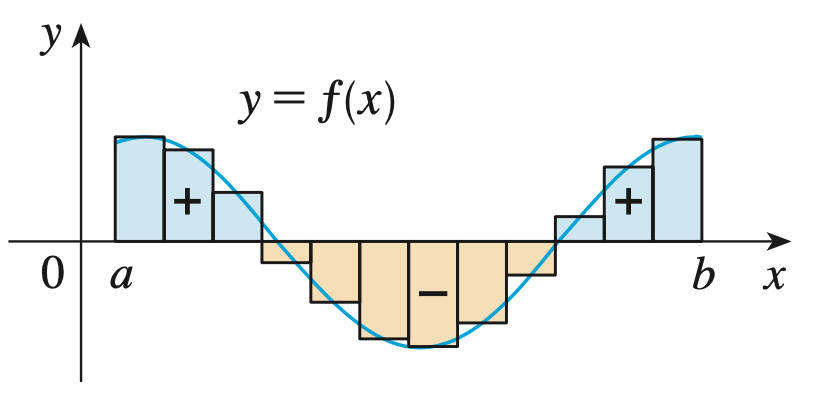
\includegraphics[scale=0.6]{fig/integral}
\caption{Integral is the net area}
\end{center}
\end{figure}

\end{frame}

\begin{frame}
\frametitle{Useful sum of powers}

\footnotesize
\everymath{\displaystyle}
\begin{itemize}
\item $\sum_{i=1}^{n}i = \dfrac{n(n+1)}{2}$
\item $\sum_{i=1}^{n}i^2 = \dfrac{n(n+1)(2n+1)}{6}$
\item $\sum_{i=1}^{n}i^3 = \left[\dfrac{n(n+1)}{2}\right]^2$
\item $\sum_{i=1}^{n}c = nc$
\item $\sum_{i=1}^{n}ca_i = c\sum_{i=1}^{n}a_i$
\item $\sum_{i=1}^{n}(a_i \pm b_i) = \sum_{i=1}^{n}a_i \pm \sum_{i=1}^{n}b_i$
\end{itemize}

\end{frame}


\begin{frame}
\frametitle{Basic properties of the definite Integral}

\footnotesize

 Suppose that $a$, $b$, $d$ are real numbers and $f$ is integrable on $[a,b]$, and $c$ is a constant.
\begin{enumerate}
\item $\ds\int_b^af(x)\,dx = \ds-\int_a^bf(x)\,dx$
\item $\ds\int_a^af(x)\,dx = 0$
\item $\ds\int_{a}^{b}c \,dx = c(b-a)$
\item $\ds\int_{a}^{b}c f(x) \,dx = c\ds\int_{a}^{b}f(x)\,dx$
\item $\ds\int_a^b(f(x) \pm g(x))\,dx= \int_a^b f(x) \,dx \pm \int_a^b g(x)\,dx$
\item $\ds\int_{a}^{b} f(x)\,dx = \int_{a}^{d}f(x)\,dx + \int_{d}^{b}f(x)\,dx$
\end{enumerate}
\end{frame}

\begin{frame}
\frametitle{Comparison properties of the definite Integral}
\footnotesize

\noindent Suppose that $a \leq b$.

\begin{enumerate}
\item If $f(x)\geq0$ for all $x$ in $[a,b]$ then $\ds \int_a^b f(x)\,dx\geq0$.

\vspace*{.3cm}

\item If $f(x)\leq g(x)$ for all $x$ in $[a,b]$ then
\[\ds \int_a^b f(x)\,dx\leq\int_a^b g(x)\,dx.\]

\vspace*{.3cm}

\item If $m\leq f(x)\leq M$ for all $x$ in $[a,b]$ then
\[m(b-a)\leq \int_a^b f(x)\,dx \leq M(b-a).\]


\vspace*{.3cm}

\item If $|f|$ is integrable on $[a,b]$ then
\[\left|\int_a^bf(x)\,dx\right|\leq\int_a^b|f(x)|\,dx.\]
\end{enumerate}
\end{frame}

\begin{frame}
\frametitle{Example}
\footnotesize
Evaluate $\ds\int_0^1 (4 + 3x^2) \, dx$ \pause

\begin{itemize}
	\item $\ds\int_0^1 (4 + 3x^2) \, dx = \ds\int_0^1 4 \, dx +  3 \ds\int_0^1 x^2 \, dx$
	\item $\ds\int_0^1 4 \, dx = 4(1-0) = 4$ (use prop. 3)
	\item $\triangle x = \dfrac{b-a}{n} = \dfrac{1 - 0}{n} = \dfrac{1}{n}, x_i^{*} = a + i\triangle{x} = 0 + i\dfrac{1}{n} = \dfrac{i}{n}$
	\item $\ds\int_0^1 x^2 \, dx =  \lim_{n\rightarrow \infty} \sum_{i=1}^{n} f(x_{i}^{*})\triangle x_{i} = \lim_{n\rightarrow \infty} \sum_{i=1}^{n} f(\dfrac{i}{n})\dfrac{1}{n} = \lim_{n\rightarrow \infty} \dfrac{1}{n} \sum_{i=1}^{n} \dfrac{i^2}{n^2} =  \lim_{n\rightarrow \infty}  \dfrac{1}{n^3} \sum_{i=1}^{n} i^2 =   \lim_{n\rightarrow \infty} \dfrac{1}{n^3} \big( \dfrac{n(n+1)(2n+1)}{6}\big) =  \lim_{n\rightarrow \infty}\dfrac{2n^3 + 3n^2 + n}{6n^3} =  \lim_{n\rightarrow \infty} \dfrac{n^3 (2 + \frac{3}{n} + \frac{1}{n^2})}{6n^3} = \frac{1}{3}$
	\item $ \ds\int_0^1 4 \, dx +  3 \ds\int_0^1 x^2 \, dx = 4 + 3(\frac{1}{3}) = 5$
\end{itemize}

\end{frame}


\begin{frame}
\frametitle{Exercises}

Evaluate the following integrals:

\begin{itemize}
	\item $\ds\int_2^5 (4 - 2x) \, dx$
	\begin{itemize}
		\item Ans: -9
	\end{itemize}
	\item $\ds\int_0^2 2x - x^3 \, dx$
	\begin{itemize}
		\item Ans: 0
	\end{itemize}
\end{itemize}

\end{frame}

\begin{frame}
\frametitle{Exercise}
\footnotesize
Evaluate $\ds\int_2^5 (4 - 2x) \, dx$ \pause

\begin{itemize}
	\item $ \ds\int_2^5 4 \, dx  -  2 \ds\int_2^5 x\, dx$
	\item $\ds\int_2^5 4 \, dx = 4(5-2) = 12$ (use prop. 3)
	\item $\triangle x = \dfrac{b-a}{n} = \dfrac{5-2}{n} = \dfrac{3}{n}, x_i^{*} = a + i\triangle{x} = 2 + i\dfrac{3}{n} = 2 + \dfrac{3i}{n}$
	\item $\ds\int_2^5 x \, dx =  \lim_{n\rightarrow \infty} \sum_{i=1}^{n} f(x_{i}^{*})\triangle x_{i} = \lim_{n\rightarrow \infty} \sum_{i=1}^{n} f(2 + \dfrac{3i}{n}) \dfrac{3}{n} = \lim_{n\rightarrow \infty}  \sum_{i=1}^{n}  (2 + \dfrac{3i}{n})\dfrac{3}{n}   =  \lim_{n\rightarrow \infty} \dfrac{3}{n}  \left( \sum_{i=1}^{n}  2 +  \dfrac{3}{n}  \sum_{i=1}^{n} i\right) = \lim_{n\rightarrow \infty} \dfrac{3}{n}  \left(2n +  \dfrac{3}{n}( \dfrac{n(n+1)}{2})\right) =  \lim_{n\rightarrow \infty} \dfrac{6n}{n} + \dfrac{9n + 9}{2n} = 6 + \frac{9}{2} + 0 = \frac{21}{2}$
	\item  $ \ds\int_2^5 4 \, dx  -  2 \ds\int_2^5 x\, dx =  12 - 2(\dfrac{21}{2}) = -9$
\end{itemize}

\end{frame}

\begin{frame}
\frametitle{Exercise}
\footnotesize
Evaluate $\ds\int_0^2 2x - x^3 \, dx$ \pause

\begin{itemize}
	\item $\triangle x = \dfrac{2}{n}, x_i^{*} = \dfrac{2i}{n}$
	\item $\ds \lim_{n\rightarrow \infty} \sum_{i=1}^{n} f(x_{i}^{*})\triangle x_{i} = \lim_{n\rightarrow \infty} \sum_{i=1}^{n} f(\dfrac{2i}{n}) \dfrac{2}{n} =  \lim_{n\rightarrow \infty} \dfrac{2}{n} \left( \sum_{i=1}^{n} 2(\dfrac{2i}{n}) - (\dfrac{2i}{n})^3\right) = \lim_{n\rightarrow \infty} \dfrac{2}{n} \left( \sum_{i=1}^{n} \dfrac{4i}{n} - \dfrac{8i^3}{n^3}\right) = \lim_{n\rightarrow \infty} \dfrac{2}{n} \left( \dfrac{4}{n}\sum_{i=1}^{n} i - \dfrac{8}{n^3}\sum_{i=1}^{n} i^3 \right) = \lim_{n\rightarrow \infty} \dfrac{2}{n} \left( \dfrac{4}{n} \cdot \dfrac{n(n+1)}{2} - \dfrac{8}{n^3} \cdot \left[\dfrac{n(n+1)}{2}\right]^2 \right) = \lim_{n\rightarrow \infty} \dfrac{8}{n^2} \cdot \dfrac{n^2 + n}{2} - \dfrac{16}{n^4} \cdot \dfrac{n^4 + n^3 + n^3 + n^2}{4} = 4 - 4 = 0$
\end{itemize}

\end{frame}

\end{document}